
\chapter{Metodologie e Strumenti Di Sviluppo}
\label{chap:metod}

\section{Metodologie di Sviluppo}
Durante lo sviluppo del progetto abbiamo utilizzato uno sviluppo Scrum\cite{scr} unito al modello incrementale, utilizzando un Scrum per quanto riguarda la distribuzione del lavoro e il rapporto con l'azienda, mentre il rilascio incrementale è stato utilizzato una volta scoperte tutte le potenzialità del Dial e il corretto funzionamento su pagine web.

\subsection{Scrum}
 
Scrum è un framework agile per la gestione del ciclo di sviluppo del software, iterativo ed incrementale, concepito per gestire progetti e prodotti software o applicazioni di sviluppo, creato e sviluppato da Ken Schwaber e Jeff Sutherland.\\

\begin{figure}[htpb!]
\center
  
\includegraphics[width=0.4\textwidth]{Scrum}
  \caption{Scrum}
\end{figure}

Scrum enfatizza tutti gli aspetti di gestione di progetto legati a contesti in cui è difficile pianificare in anticipo. Vengono utilizzati meccanismi propri di un "processo di controllo empirico", in cui cicli di feedback che ne costituiscono le tecniche di management fondamentali risultano in opposizione alla gestione basata sul concetto tradizionale di command-and-control. Il suo approccio alla pianificazione e gestione di progetti è quello di portare l'autorità decisionale al livello di proprietà e certezze operative.\\

Sono 3 i ruoli che vengono individuati nella metodologia Scrum: \emph{Product Owner}, \emph{Scrum Master} e \emph{Team di Sviluppo}:

\begin{itemize}
\item Il \textbf{Product Owner} definisce il lavoro da svolgere e l'ordine con cui viene completato. Raccoglie la voce degli stakeholder (clienti, management e chiunque abbia un interesse nel prodotto), le necessità dell'utente finale, i requisiti del mercato e sulla base di questi elementi stabilisce le priorità di sviluppo per il Team Scrum.
\item Lo \textbf{Scrum Master} è il responsabile del processo, e un leader a servizio (servant-leader) dello Scrum Team. Conoscitore esperto della metodologia Scrum, sa come applicarla e si assicura che il Team comprenda e segua le regole che la caratterizzano, perché il progetto abbia successo. Inoltre favorisce il lavoro del Team di Sviluppo, rimuovendo ostacoli, organizzando meeting di confronto, e soprattutto proteggendolo da ogni possibile distrazione: ogni membro del gruppo deve poter lavorare al 100 per 100 sullo sviluppo, e lo Scrum Master si assicura che questo avvenga.
\item Il \textbf{Team di Sviluppo} è la squadra di lavoro, composta da 3 a 9 persone. Anche lo Scrum Master può far parte del Team di Sviluppo. Chi concretamente porta a termine gli Sprint e fornisce le funzionalità da implementare è questo insieme coordinato di persone, autogestito e cross-funzionale.
\end{itemize}

Per quanto riguarda il nostro progetto, abbiamo applicato il framework Scrum con i ruoli definiti nel seguente schema:
\begin{itemize}
\item \textbf{Product Owner}: Luca Mazzuferi
\item \textbf{Scrum Master}: Marco Allegrezza, Diego Bonura
\item \textbf{Team di Sviluppo}: Daniele Moschini, Michele Benedetti
\end{itemize}

\newpage
\subsection{Rilascio Incrementale}

Per \textbf{modello incrementale}\cite{rin} si intende, nell'ambito dell'ingegneria del software, un modello di sviluppo di un progetto software basato sulla successione dei seguenti passi principali:

\begin{itemize}
\item Pianificazione
\item Analisi dei requisiti
\item Progetto
\item Implementazione
\item Prove
\item Valutazione
\end{itemize}

Questo ciclo può essere ripetuto diverse volte, in cui ogni "incremento" riduce il rischio di fallimento e produce nuovo valore. Il ciclo viene ripetuto fino a che la valutazione del prodotto diviene soddisfacente rispetto ai requisiti previsti.\\

L'utilizzo del modello incrementale è consigliabile quando si ha, fin dall'inizio della progettazione, una visione abbastanza chiara dell'intero progetto, perché occorre fare in modo che la realizzazione della generica versione k risulti utile per la realizzazione della versione k+1.\\

Un approccio incrementale è particolarmente indicato in tutti quei casi in cui la specifica dei requisiti risulti particolarmente difficoltosa e di difficile stesura (semi)formale. L'uso di questo modello di sviluppo favorisce la creazione di prototipi, ovvero parti di applicazione funzionanti, che a loro volta favoriscono il dialogo con il cliente e la validazione dei requisiti.

\begin{figure}[htpb!]
\center
  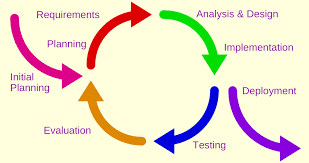
\includegraphics[width=0.6\textwidth]{RilascioIncrementale}
  \caption{Rilascio Incrementale}
\end{figure}

\newpage
\section{Strumenti utilizzati}

Durante lo sviluppo del progetto, sono state utilizzate varie tecnologie, strumenti, linguaggi e relativi framework che verranno dettagliatamente descritti di seguito.

\subsection{Microsoft Dial}

\begin{figure}[htpb!]
\center
  \includegraphics[width=0.4\textwidth]{Dial}
  \caption{Microsoft Dial}
\end{figure}

Il Microsoft Surface Dial\cite{dial} é un dispositivo di rotazione proprietario Microsoft, ideato per l'utilizzo con la mano secondaria durante le attivitá di progettazione e modifica dati. Composto da un sensore laser che permette di calcolare 3600 punti di precisione grazie alla sua riflessione e da un sistema di vibrazione haptico che restituisce un feedback tattile durante l'utilizzo. Nella parte inferiore presenta un plate in silicone ideato per generare la giusta aderenza durante il contatto con display inclinati.\\

\begin{figure}[htpb!]
	\begin{minipage}{0.35\textwidth}
		\centering
		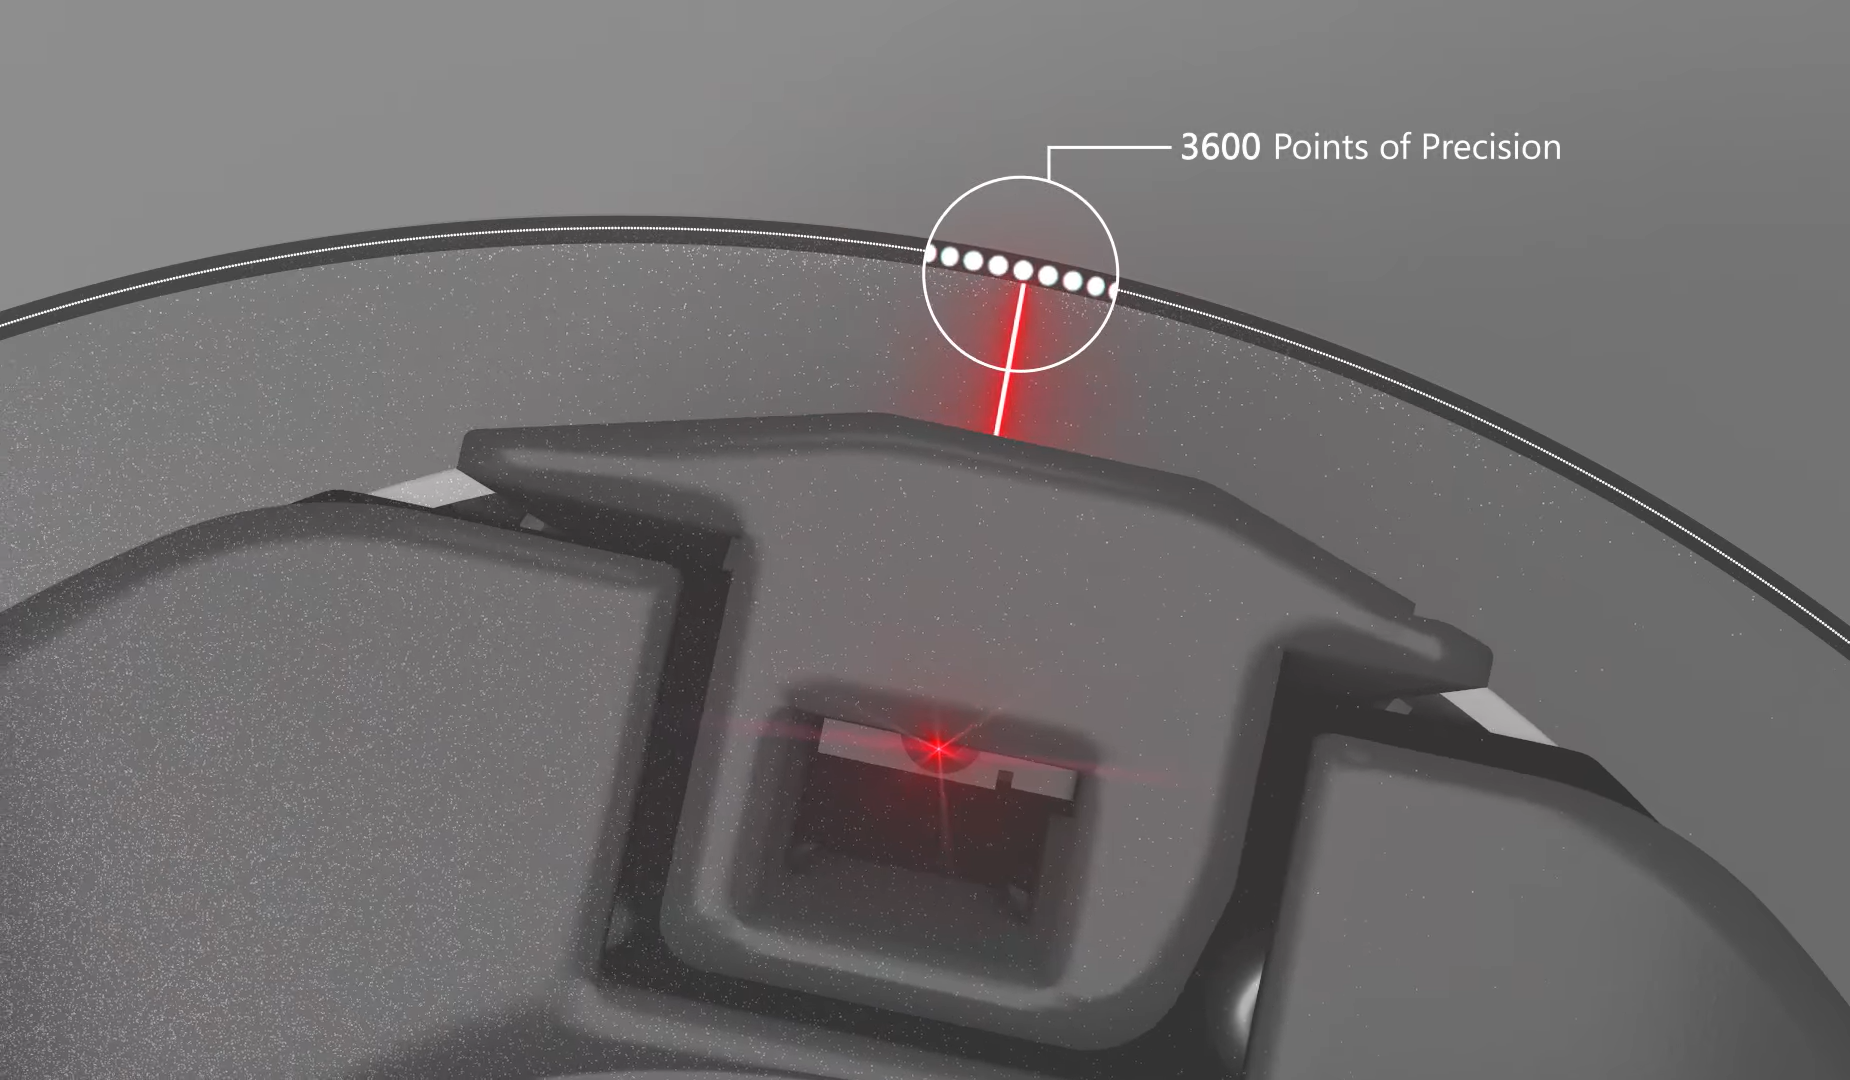
\includegraphics[width=0.9\textwidth]{DialPoint}
		\caption{Dial laser point}
    \end{minipage}\hfill
    \begin{minipage}{0.65\textwidth}
		\centering
		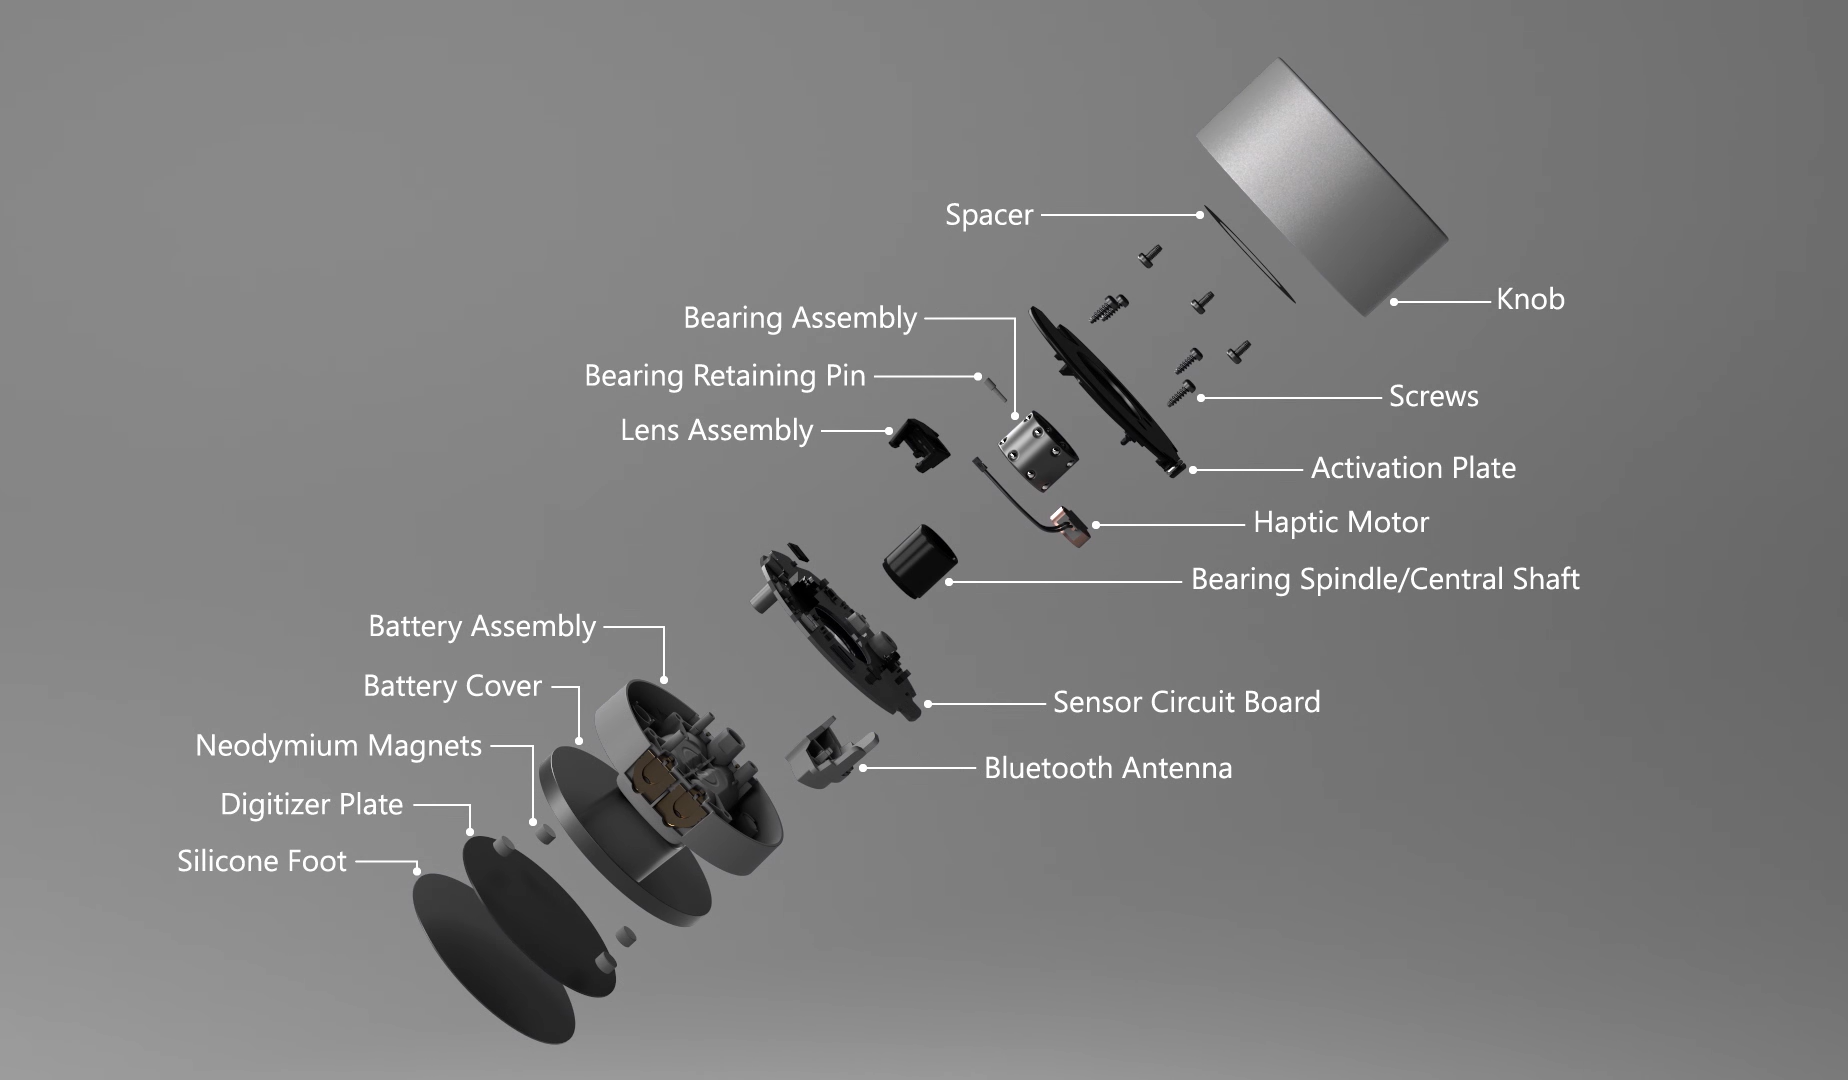
\includegraphics[width=0.9\textwidth]{DialEsploso}
		\caption{Dial Esploso}
    \end{minipage}
\end{figure}

Un ulteriore funzionalitá é rappresentata dal riconoscimento della posizione e del contatto del dispositivo con display touch-screen supportati, che avviene attraverso la presenza di quattro magneti al \emph{Neodymium}. 
\newpage
\subsection{Surface Pro 6}
\begin{figure}[htpb!]
\center
  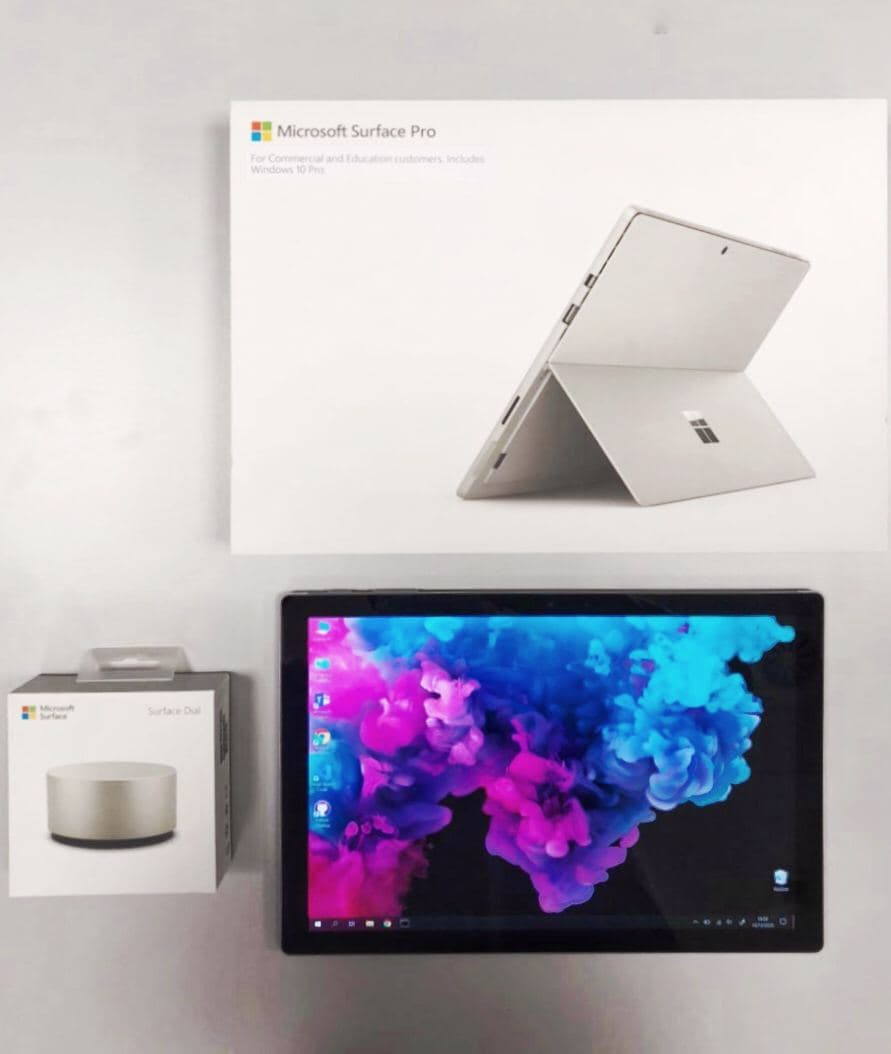
\includegraphics[width=0.3\textwidth]{Hardware}
  \caption{Surface Pro 6}
\end{figure}
Il Surface Pro 6\cite{sur} è un computer tablet 2-in-1 sviluppato da Microsoft . È la sesta generazione di Surface Pro ed è stato annunciato insieme al Surface Laptop 2 il 2 ottobre 2018 in un evento a New York.
\subsection{Aulos}
\begin{figure}[htpb!]
\center
  
\includegraphics[width=0.3\textwidth]{LogoAulos}
  \caption{Aulos}
\end{figure}
AULOS \cite{aul} è un framework ad uso interno per la standardizzazione dello sviluppo delle commesse.
Gli obiettivi principali di questo framework sono:
\begin{itemize}
\item rendere standard e subito disponibili quelle funzionalità che sono di frequente implementazione tra le commesse;
\item fornire uno standard UI e UX che sia ben riconoscibile, ma soprattutto coerente tra commesse diverse;
\item garantire l’interoperabilità tra tecnologie diverse.
\end{itemize}

AULOS fa uso di tecnologie web come Angular per il proprio frontend, mentre il backend – a cui esso si aggancia e che regola il funzionamento della commessa – può essere scritto in più linguaggi come C\# e LabView.
Da qui si nota come AULOS sia anche uno standard di comunicazione: l’utilizzo di API apre alla possibilità di sviluppare il backend nella tecnologia che meglio si sposa con il problema da risolvere.
\newpage
\subsection{Angular}
\begin{figure}[htpb!]
\center
  
\includegraphics[width=0.2\textwidth]{LogoAngular}
  \caption{Angular}
\end{figure}
Angular 2+\cite{ang} (o semplicemente Angular) è un framework open source per lo sviluppo di applicazioni web con licenza MIT, evoluzione di AngularJS. Sviluppato principalmente da Google, la sua prima release è avvenuta il 14 settembre 2016.Angular è stato completamente riscritto rispetto a AngularJS e le due versioni non sono compatibili. Il linguaggio di programmazione usato per AngularJS è JavaScript mentre quello di Angular è TypeScript. Le applicazioni sviluppate in Angular vengono eseguite interamente dal web browser dopo essere state scaricate dal web server (elaborazione lato client). Questo comporta il risparmio di dover spedire indietro la pagina web al web-server ogni volta che c'è una richiesta di azione da parte dell'utente. Il codice generato da Angular gira su tutti i principali web browser moderni quali ad esempio Chrome, Microsoft Edge, Opera, Firefox, Safari ed altri. Angular è stato progettato per fornire uno strumento facile e veloce per sviluppare applicazioni che girano su qualunque piattaforma inclusi smartphone e tablet. Infatti le applicazioni web in Angular in combinazione con il toolkit open source Bootstrap diventano responsive, ossia il design del sito web si adatta in funzione alle dimensioni del dispositivo utilizzato. È in corso di sviluppo un altro toolkit di design responsivo, Flex Layout, più semplice da usare rispetto a Bootstrap e concepito appositamente per Angular. Altro toolkit che facilita la progettazione in Angular è Angular Material, una serie di componenti che permette di creare una pagina web molto velocemente: con l'utilizzo combinato di Flex Layout ed Angular Material si possono creare siti e applicazioni web responsive molto avanzate basate su Angular.
\subsection{TypeScript}
\begin{figure}[htpb!]
\center
  
\includegraphics[width=0.4\textwidth]{LogoTypescript}
  \caption{Typescript}
\end{figure}
TypeScript\cite{typ} è un linguaggio di programmazione open source sviluppato da Microsoft. Si tratta di un Super-set di JavaScript che basa le sue caratteristiche su ECMAScript 6; capo del progetto è Anders Hejlsberg. Il linguaggio estende la sintassi di JavaScript in modo che qualunque programma scritto in JavaScript sia anche in grado di
16
funzionare con TypeScript senza nessuna modifica. È stato progettato per lo sviluppo di grandi applicazioni ed è destinato a essere compilato in JavaScript per poter essere interpretato da qualunque web browser o app.
\subsection{HTML}
\begin{figure}[htpb!]
\center
  
\includegraphics[width=0.2\textwidth]{LogoHTML}
  \caption{HTML}
\end{figure}
L'HTML\cite{html} è un linguaggio di pubblico dominio, la cui sintassi è stabilita dal World Wide Web Consortium (W3C). È derivato dall'SGML, un metalinguaggio finalizzato alla definizione di linguaggi utilizzabili per la stesura di documenti destinati alla trasmissione in formato elettronico. La versione attuale, la quinta, è stata rilasciata dal W3C nell'ottobre 2014. Il motivo principale che ha spinto il W3C e i suoi membri a sviluppare HTML5 è stata la necessità di fornire direttamente le funzionalità che in precedenza erano fruibili tramite estensioni proprietarie all'esterno dei browser, come Adobe Flash e simili. Un secondo obiettivo che gli sviluppatori si erano prefissati era quello di garantire una maggiore compatibilità tra i diversi browser, indipendentemente dalla piattaforma software utilizzata, e principalmente mirata all'espansione dei dispositivi mobili.
\subsection{KendoUI}
\begin{figure}[htpb!]
\center
  
\includegraphics[width=0.3\textwidth]{LogoKendo}
  \caption{KendoUI}
\end{figure}
Kendo UI\cite{ken} e un framework integrale di interfaccia utente HTML5 per costruire applicazioni e siti web interattivi e ad alte prestazioni.
\newpage
\subsection{Microsoft UWP}
\begin{figure}[htpb!]
\center
  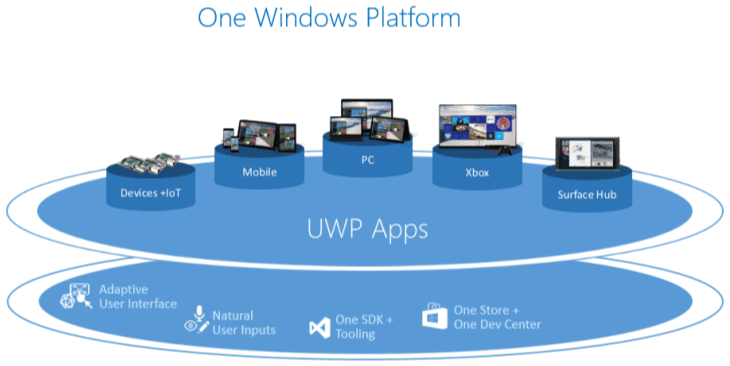
\includegraphics[width=0.45\textwidth]{LogoUWP}
  \caption{Microsoft UWP}
\end{figure}
UWP\cite{uwpdoc} è uno dei numerosi modi per creare applicazioni client per Windows. Le app UWP usano le API WinRT per offrire potenti funzionalità avanzate di interfaccia utente e asincrone, ideali per i dispositivi connessi a Internet.
Per scaricare gli strumenti necessari per iniziare a creare le app UWP, vedere Effettuare la configurazione e quindi Scrivere la prima app ed è la soluzione ideale per creare app che vengono eseguite nei dispositivi Windows 10 e possono essere combinate con altre piattaforme. Le app UWP possono usare le API Win32 e le classi .NET (vedere Set di API per le app UWP, DLL per le app UWP e .NET per le app UWP).Il progetto di sviluppo Microsoft continua a evolversi e, insieme a iniziative come WinUI, MSIX e Project Reunion, UWP rappresenta uno strumento potente per la creazione di app client.
Un'app UWP è:
\begin{itemize}
\item Sicura: le app UWP dichiarano le risorse del dispositivo e i dati a cui accedono. L'utente deve autorizzare tale accesso.
\item In grado di usare un'API comune in tutti i dispositivi che eseguono Windows 10.
\item In grado di usare funzionalità specifiche del dispositivo e di adattare l'interfaccia utente alle dimensioni, alle risoluzioni e ai DPI dello schermo di dispositivi diversi.
\item Disponibile nel Microsoft Store in tutti i dispositivi (o solo a quelli specificati) che eseguono Windows 10. Il Microsoft Store offre diversi modi per realizzare profitti con un'app.
\item In grado di essere installata e disinstallata senza rischio o danni per il computer.
\item Coinvolgente: è possibile usare riquadri animati, notifiche push e attività utente che interagiscono con Sequenza temporale di Windows e la funzionalità di ripristino della ricerca dal punto in cui è stata interrotta di Cortana per coinvolgere gli utenti.
\item Programmabile in C\#, C++, Visual Basic e Javascript. Per l'interfaccia utente usare WinUI, XAML, HTML o DirectX
\end{itemize}
\subsection{Microsoft WebView}
Una WebView\cite{webview} integra all'interno di un' applicazione una visualizzazione che esegue il rendering di contenuto web tramite il motore di rendering di Microsoft Edge nel quale possono comparire anche collegamenti ipertestuali funzionanti.
Metodi utilizzati:
\begin{itemize}
\item \emph{AddWebAllowedObject(String, Object)}\cite{awao} Permette di iniettare oggetti runtime nativi windows come parametri globali del documento all'interno della WebView
\item \emph{InvokeScriptAsync(String, IEnumerable<String>)}\cite{isa} Permette l'invio di script specifici alla pagina web caricata con argomenti specifici come azione asincrona. 
\end{itemize}

\subsection{C\#}
\begin{figure}[htpb!]
\center
  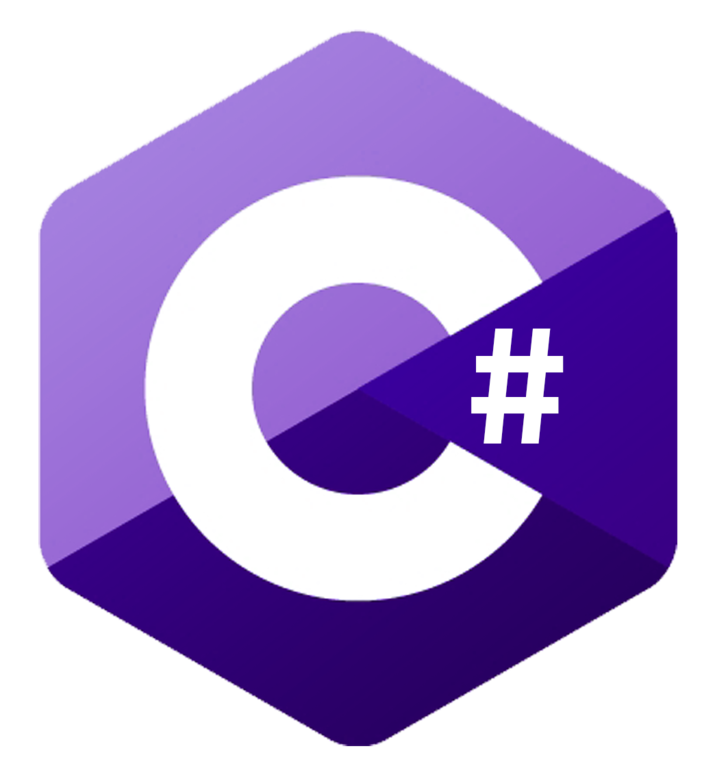
\includegraphics[width=0.2\textwidth]{LogoC}
  \caption{C\#}
\end{figure}
Il C\#\cite{cs} è un linguaggio di programmazione orientato agli oggetti sviluppato da Microsoft all'interno dell'iniziativa .NET, e successivamente approvato come standard dalla ECMA (ECMA-334) e ISO (norma ISO/IEC 23270).
La sintassi e struttura del C\# prendono spunto da vari linguaggi nati precedentemente, in particolare Delphi, C++, Java e Visual Basic.
\subsection{Libreria RadialController}
La libreria RadialController\cite{rad} e le API correlate consentono di personalizzare sia il menù dei comandi integrato che l'esperienza di interazione supportata dall’ app.
Metodi utilizzati:
\begin{itemize}


\item RadialController.CreateForCurrentView()\\
Metodo statico che consente di ricevere un oggetto della classe RadialController creato appositamente per il contesto in cui gira l’applicazione (Dial utilizzato, versione del sistema operativo, tipo di hardware, ...)
\item .CreateFromIcon("Sample", icon)\\
Metodo che consente di creare un RadialControllerMenuItem ovvero un oggetto che inserito all’interno del menu verrà visualizzato e consentirà di svolgere un determinato comportamento quando selezionato.
\item .Menu.Items.
\begin{itemize}
\item Add(RadialControllerMenuItem item)
\item Inserisce il RadialControllerMenuItem all’interno del menu.
\item CreateFromKnownIcon(string displayText, RadialControllerMenuKnownIcon value)
\item Crea un oggetto di tipo RadialControllerMenuItem da un’icona già presente nella libreria.
\item CreateFromIcon(string displayText, RandomAccessStreamReference icon)
\item Crea un oggetto di tipo RadialControllerMenuItem da un’icona presente negli assets
\item CreateFromFontGlyph(string displayText, string glyph, string fontFamily)
\item Crea un oggetto di tipo RadialControllerMenuItem da un font installato nel sistema / inserito nell’app, e da un codice esadecimale ad esso associato
\end{itemize}
\end{itemize}
Eventi utilizzati:
\begin{itemize}
\item radialController.ButtonClicked\\
Evento che informa della pressione breve del dispositivo Dial.
\item radialController.ButtonPressed\\
Evento che informa della pressione prolungata del dispositivo Dial
\item radialController.RotationChanged\\
Evento che informa della rotazione del dispositivo Dial
\item .ScreenContactStarted\\
Evento che informa del posizionamento del Dial su schermo
\item .ScreenContactContinued\\
Evento che informa sull’utilizzo del Dial su schermo
\item .ScreenContactEnded\\
Evento che informa sulla fine del posizionamento su schermo
\end{itemize}
API correlate\\
RadialControllerConfiguration è una classe correlata alla classe RadialController e permette di configurare l’oggetto della medesima classe modificando le sue proprietà.\\
SetDefaultMenuItems consente di scegliere tra le voci di menù già predisposte dalla libreria quale inserire nel menù.

\newpage
\subsection{Git}
\begin{figure}[htpb!]
\center
  
\includegraphics[width=0.2\textwidth]{LogoGit}
  \caption{Git}
\end{figure}
Un sistema di controllo di versione\cite{git} distribuito o decentralizzato (o DVCS da Distributed Version Control System) è una tipologia di controllo di versione che permette di tenere traccia delle modifiche e delle versioni apportate al codice sorgente del software, senza la necessità di dover utilizzare un server centrale, come nei casi classici.

Con questo sistema gli sviluppatori possono collaborare individualmente e parallelamente non connessi su di un proprio ramo (branch) di sviluppo, registrare le proprie modifiche (commit) ed in seguito condividerle con altri o unirle (merge) a quelle di altri, il tutto senza bisogno del supporto di un server centralizzato. Questo sistema permette diverse modalità di collaborazione, proprio perché il server è soltanto un mero strumento d'appoggio.
\subsection{GitLab}
\begin{figure}[htpb!]
\center
  
\includegraphics[width=0.2\textwidth]{LogoGitLab}
  \caption{GitLab}
\end{figure}
GitLab\cite{gitl} è una piattaforma web open source che permette la gestione di repository Git e di funzioni trouble ticket. Appartiene a GitLab Inc.
Come tutti i software di controllo versione, GitLab permette la creazione di repository pubblici o privati, in cui gli sviluppatori possono caricare il proprio codice e gestire le modifiche alle varie
11
versioni in contemporanea al lavoro di più persone. In GitLab è possibile lavorare parallelamente ad altre persone sullo stesso progetto senza generare conflitti, caricare il proprio lavoro nel repository remoto (operazione di push) e poter unire alla fine le modifiche di tutti in un unico progetto (operazione di merge). È possibile fare delle merge request per il proprietario del repository, oltre al tracciamento degli issue, la possibilità di scrivere commenti e allegare documenti. GitLab mette a disposizione diverse funzionalità a seconda del tipo di abbonamento e del prezzo pagato. È comunque possibile utilizzarlo gratuitamente, seppur con delle limitazioni.

\newpage
\subsection{Miro}
\begin{figure}[htpb!]
\center
  
\includegraphics[width=0.3\textwidth]{LogoMiro}
  \caption{Miro}
\end{figure}
Miro\cite{miro} è la piattaforma di lavagna collaborativa online per il lavoro moderno, consentendo a team collocati, distribuiti e remoti di comunicare e collaborare tra formati, strumenti, canali e fusi orari, senza i vincoli di posizione fisica, spazio per riunioni e lavagna
\subsection{Teams}
\begin{figure}[htpb!]
\center
  
\includegraphics[width=0.4\textwidth]{LogoTeams}
  \caption{Teams}
\end{figure}
Microsoft Teams\cite{mt} è una piattaforma di comunicazione e collaborazione unificata che combina chat di lavoro persistente, teleconferenza, condivisione di contenuti (incluso lo scambio e il lavoro simultaneo sui file) e integrazione delle applicazioni. Il servizio si integra con la suite di produttività per l'ufficio in abbonamento di Microsoft 365 e include estensioni che possono integrarsi con prodotti non Microsoft.
\subsection{Trello}
\begin{figure}[htpb!]
\center
  
\includegraphics[width=0.2\textwidth]{LogoTrello}
  \caption{Trello}
\end{figure}
Trello\cite{tr} è un software gestionale in stile Kanban basato sul web che consente agli utenti la possibilità di creare le loro schede attività con più colonne e scambiare le attività tra di loro. In genere le colonne sono organizzate in stati dell'attività: Da fare, In corso, Fatto. Il software è utilizzabile per uso personale e aziendale. Ha una varietà di possibilità di impiego, come la gestione immobiliare, la gestione di progetti software, i bollettini scolastici, la pianificazione delle lezioni, la contabilità, il web design, i giochi e la gestione di casi legali.

\newpage
\subsection{Visual Studio}
\begin{figure}[htpb!]
\center
  
\includegraphics[width=0.2\textwidth]{LogoVS}
  \caption{Visual Studio}
\end{figure}
Microsoft Visual Studio\cite{vs} (o più comunemente Visual Studio) è un ambiente di sviluppo integrato (Integrated development environment o IDE) sviluppato da Microsoft.
Visual Studio è multilinguaggio e attualmente supporta la creazione di progetti per varie piattaforme, tra cui anche Mobile e Console. È possibile creare ed utilizzare estensioni e componenti aggiuntivi.
Visual Studio, nelle sue ultime versioni da quando è nata la piattaforma .NET, supporta diversi linguaggi di programmazione tra cui C\#, Visual Basic .Net e C++. Nelle passate edizioni era disponibile anche il supporto a J\#. Visual Studio è incompatibile col linguaggio Java da cui comunque il linguaggio J\# aveva preso forte ispirazione.
Come il suo predecessore, Visual Studio integra la tecnologia IntelliSense che permette di correggere eventuali errori sintattici, e anche alcuni logici, senza compilare l'applicazione, possiede un debugger interno per il rilevamento e la correzione degli errori logici nel codice in runtime e fornisce diversi strumenti per l'analisi delle prestazioni.Si integra nativamente con l'ambiente di sviluppo di gruppo Team Foundation Server che, tra le altre cose, permette di effettuare operazioni di versioning del codice.
Visual Studio dispone di diversi template per ciascun linguaggio di programmazione supportato, ad esempio Applicazione desktop, libreria di classi, servizio di Windows e diversi sottomenu che consentono di indirizzarsi sulla piattaforma per cui si desidera sviluppare. Tra queste: Microsoft Azure, Windows Store e smartphone Android e iOS
17
grazie all'integrazione con Xamarin. Le applicazioni desktop in Visual Basic .NET e Visual C\# possono essere a loro volta sviluppate utilizzando la classica tecnologia dei form oppure Windows Presentation Foundation.Nelle due versioni 2015 e 2017 il programma si è notevolmente ingrandito fino a una dimensione di circa 80 GB per un'installazione completa. Infatti sono state introdotte nuove funzioni come il supporto per gli strumenti nativi Python e applicazioni Linux, l'integrazione con Unity per lo sviluppo di videogiochi, il simulatore Android e iOS, la possibilità di gestire e modificare cursori, icone e immagini all'interno dell'applicazione.
L'interfaccia grafica dell'IDE dispone di una casella degli strumenti, disponibile solo per VB.NET, C\# e ASP.NET, da cui è possibile trascinare i controlli (tra cui TextBox, Label, ImageBox, Button) direttamente nel form del programma che si sta progettando e modificarne l'aspetto senza necessariamente passare dal codice. Attraverso gli eventi si gestisce il comportamento di questi componenti.Inoltre Visual Studio consente di reperire e installare template e componenti aggiuntivi di terze parti dal Web per ottenere ulteriori funzionalità. Per esempio esistono estensioni che introducono il supporto per il linguaggio PHP.
\subsection{Remote Tools}
Remote Tool\cite{rd} è uno strumento messo a disposizione da Microsoft che permette il debug di applicazioni UWP su dispositivi remoti collegati all'interno della rete corrente.
\subsection{Visual Studio Code}
\begin{figure}[htpb!]
\center
  
\includegraphics[width=0.4\textwidth]{LogoVSCode}
  \caption{Visual Studio Code}
\end{figure}
Visual Studio Code\cite{vsc} è un editor di codice sorgente sviluppato da Microsoft per Windows, Linux e macOS. Include il supporto per debugging, un controllo per Git integrato, Syntax highlighting, IntelliSense, Snippet e refactoring del codice. Sono personalizzabili il tema dell'editor, le scorciatoie da tastiera e le preferenze. È un software libero e gratuito, anche se la versione ufficiale è sotto una licenza proprietaria.Visual Studio Code è basato su Electron, un framework con cui è possibile sviluppare applicazioni Node.js.
Visual Studio Code è un editor di codice sorgente che può essere usato con vari linguaggi di programmazione, tra cui la famiglia di linguaggi C (C, C++, C\#), F\#, HTML e altri linguaggi web, tra cui PHP, Java, Ruby e molti altri. Incorpora un insieme di funzioni che variano a seconda del linguaggio che si sta usando, come mostrato nella tabella seguente. Molte delle funzioni di Visual Studio Code non sono accessibili attraverso menu o interfacce utente, ma piuttosto attraverso una finestra di comando o un file .json, ad esempio le preferenze dell'utente. La finestra di comando è un'Interfaccia a riga di comando, che scompare appena l'utente clicca in un'area al di fuori della finestra o preme una serie di tasti per interagire con qualcosa al di fuori di essa.
In quanto editor di codice sorgente, Visual Studio Code permette la modifica della Codifica di caratteri, il carattere inizio nuova linea (si può scegliere tra LF e CR+LF) e il linguaggio di programmazione del documento che si sta modificando.
